\chapter{System Design}

\begin{figure}[H]
    \centering
    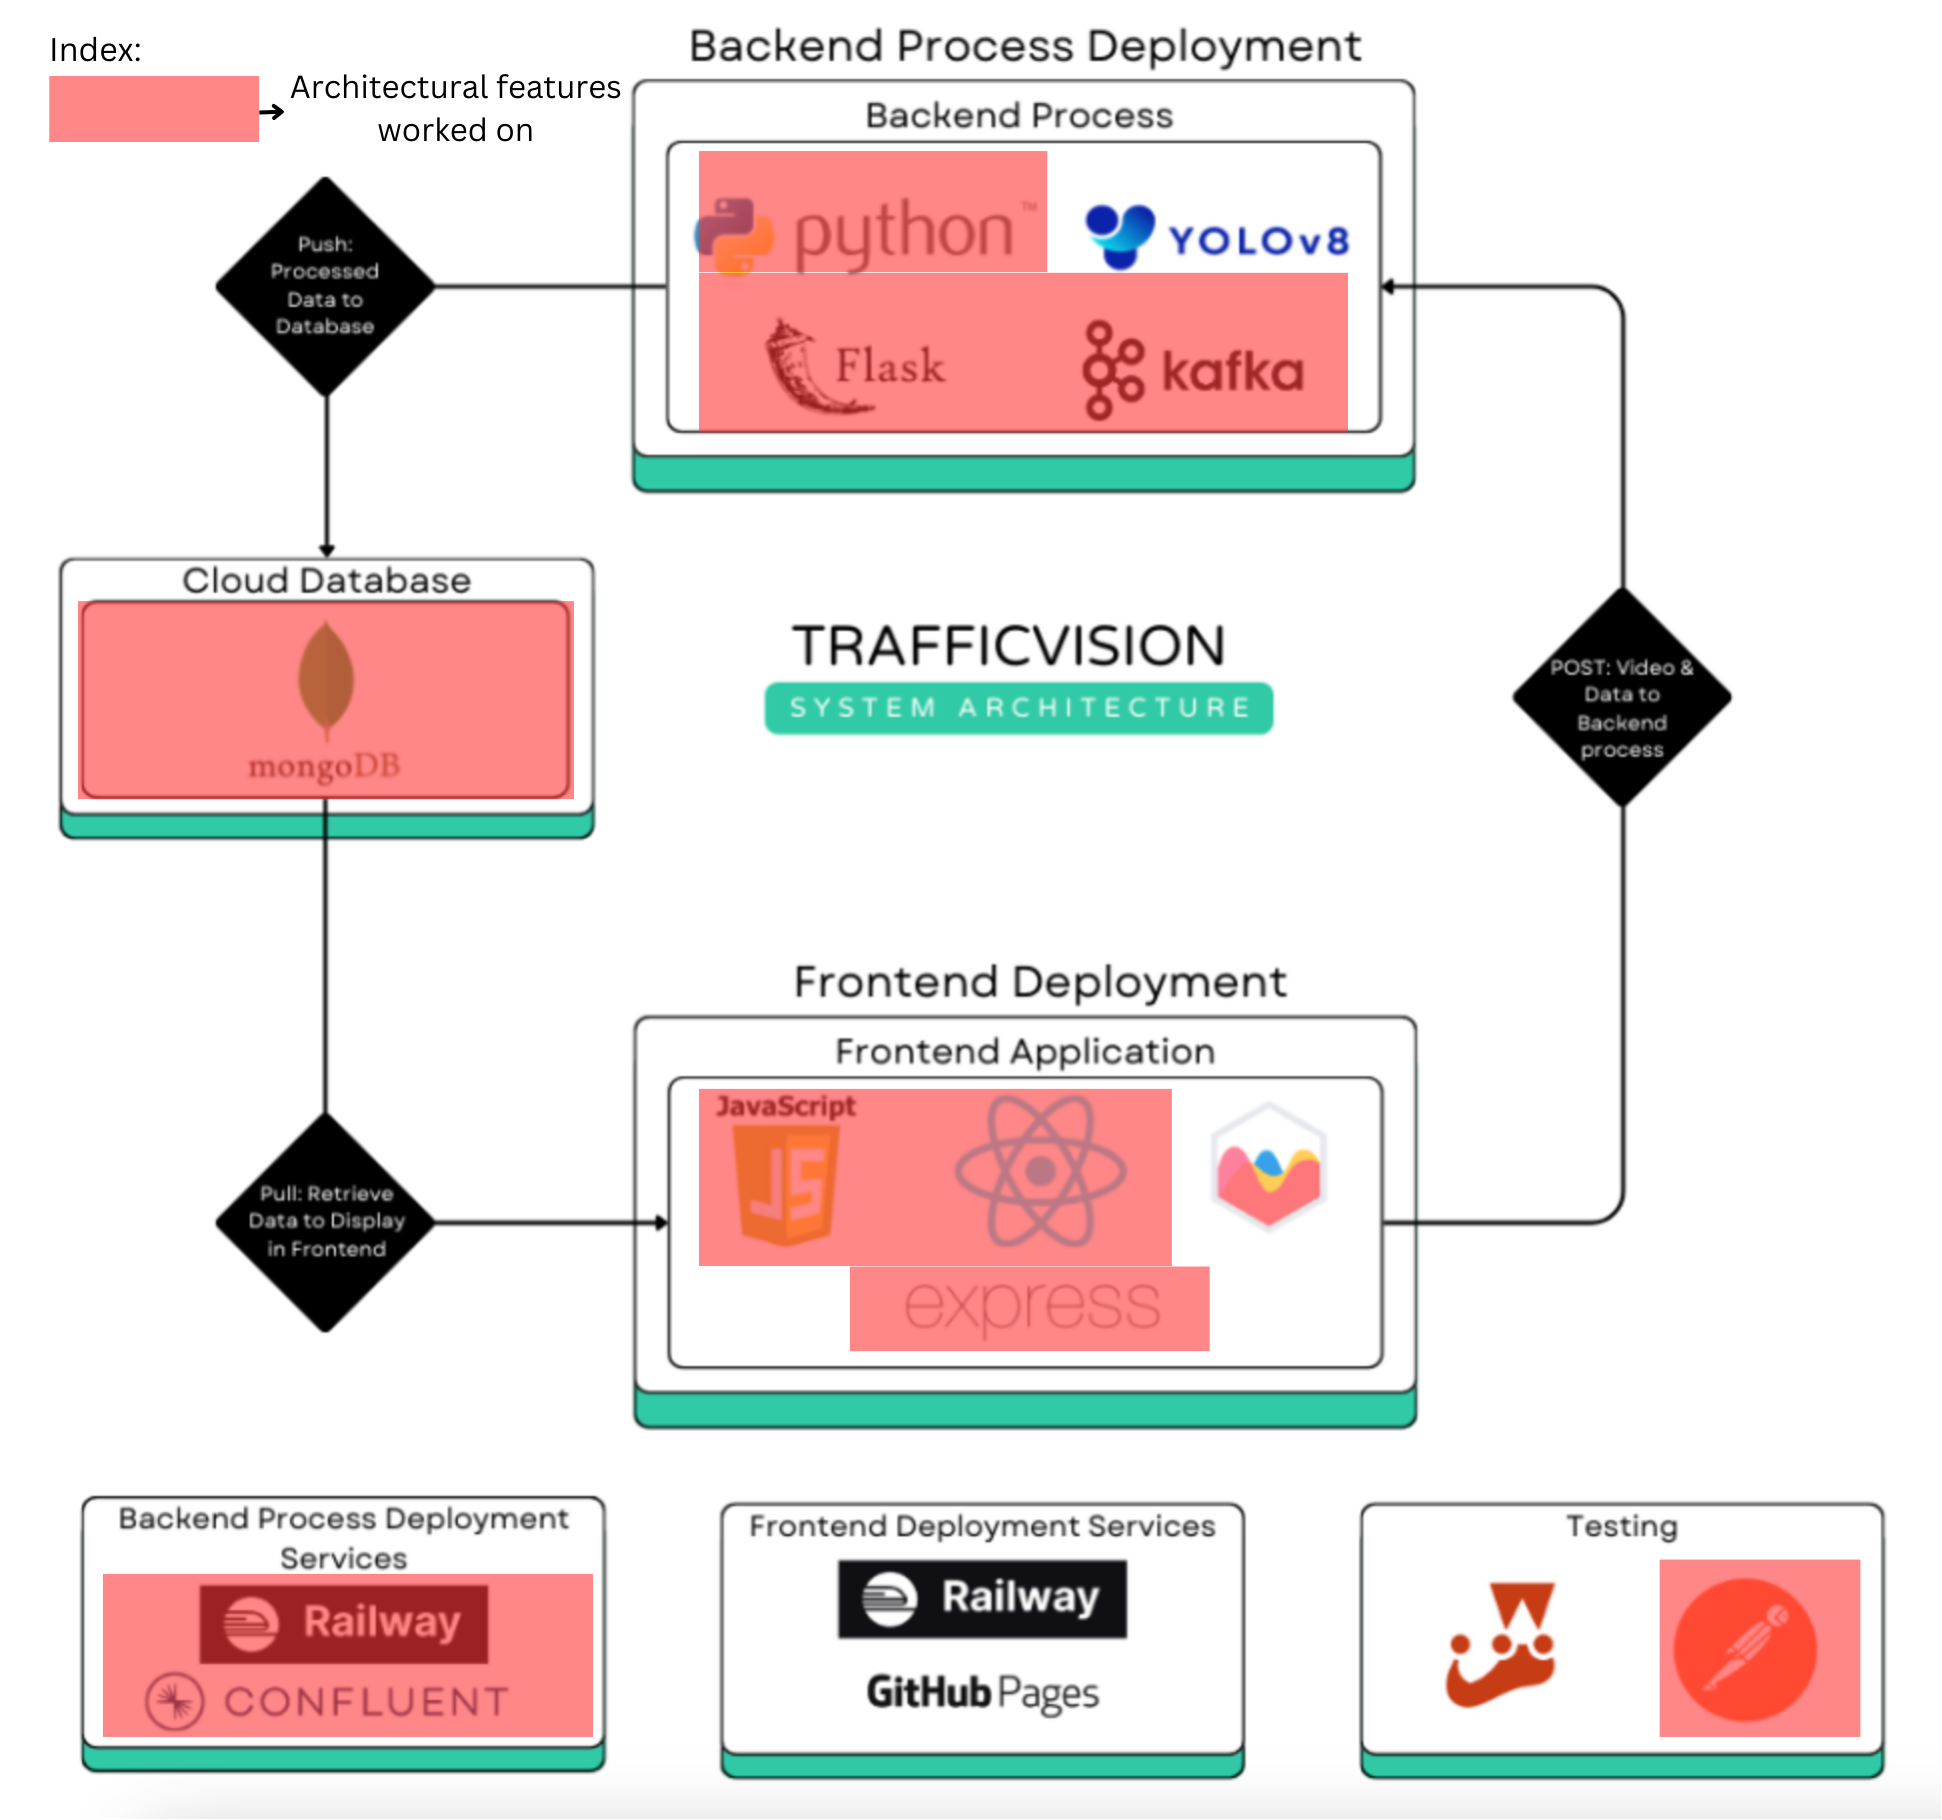
\includegraphics[width=0.9\textwidth]{images/architecture.png}
    \caption{System Architecture.}
    \label{image:sysArchitecture}
\end{figure}

\begin{figure}[H]
    \centering
    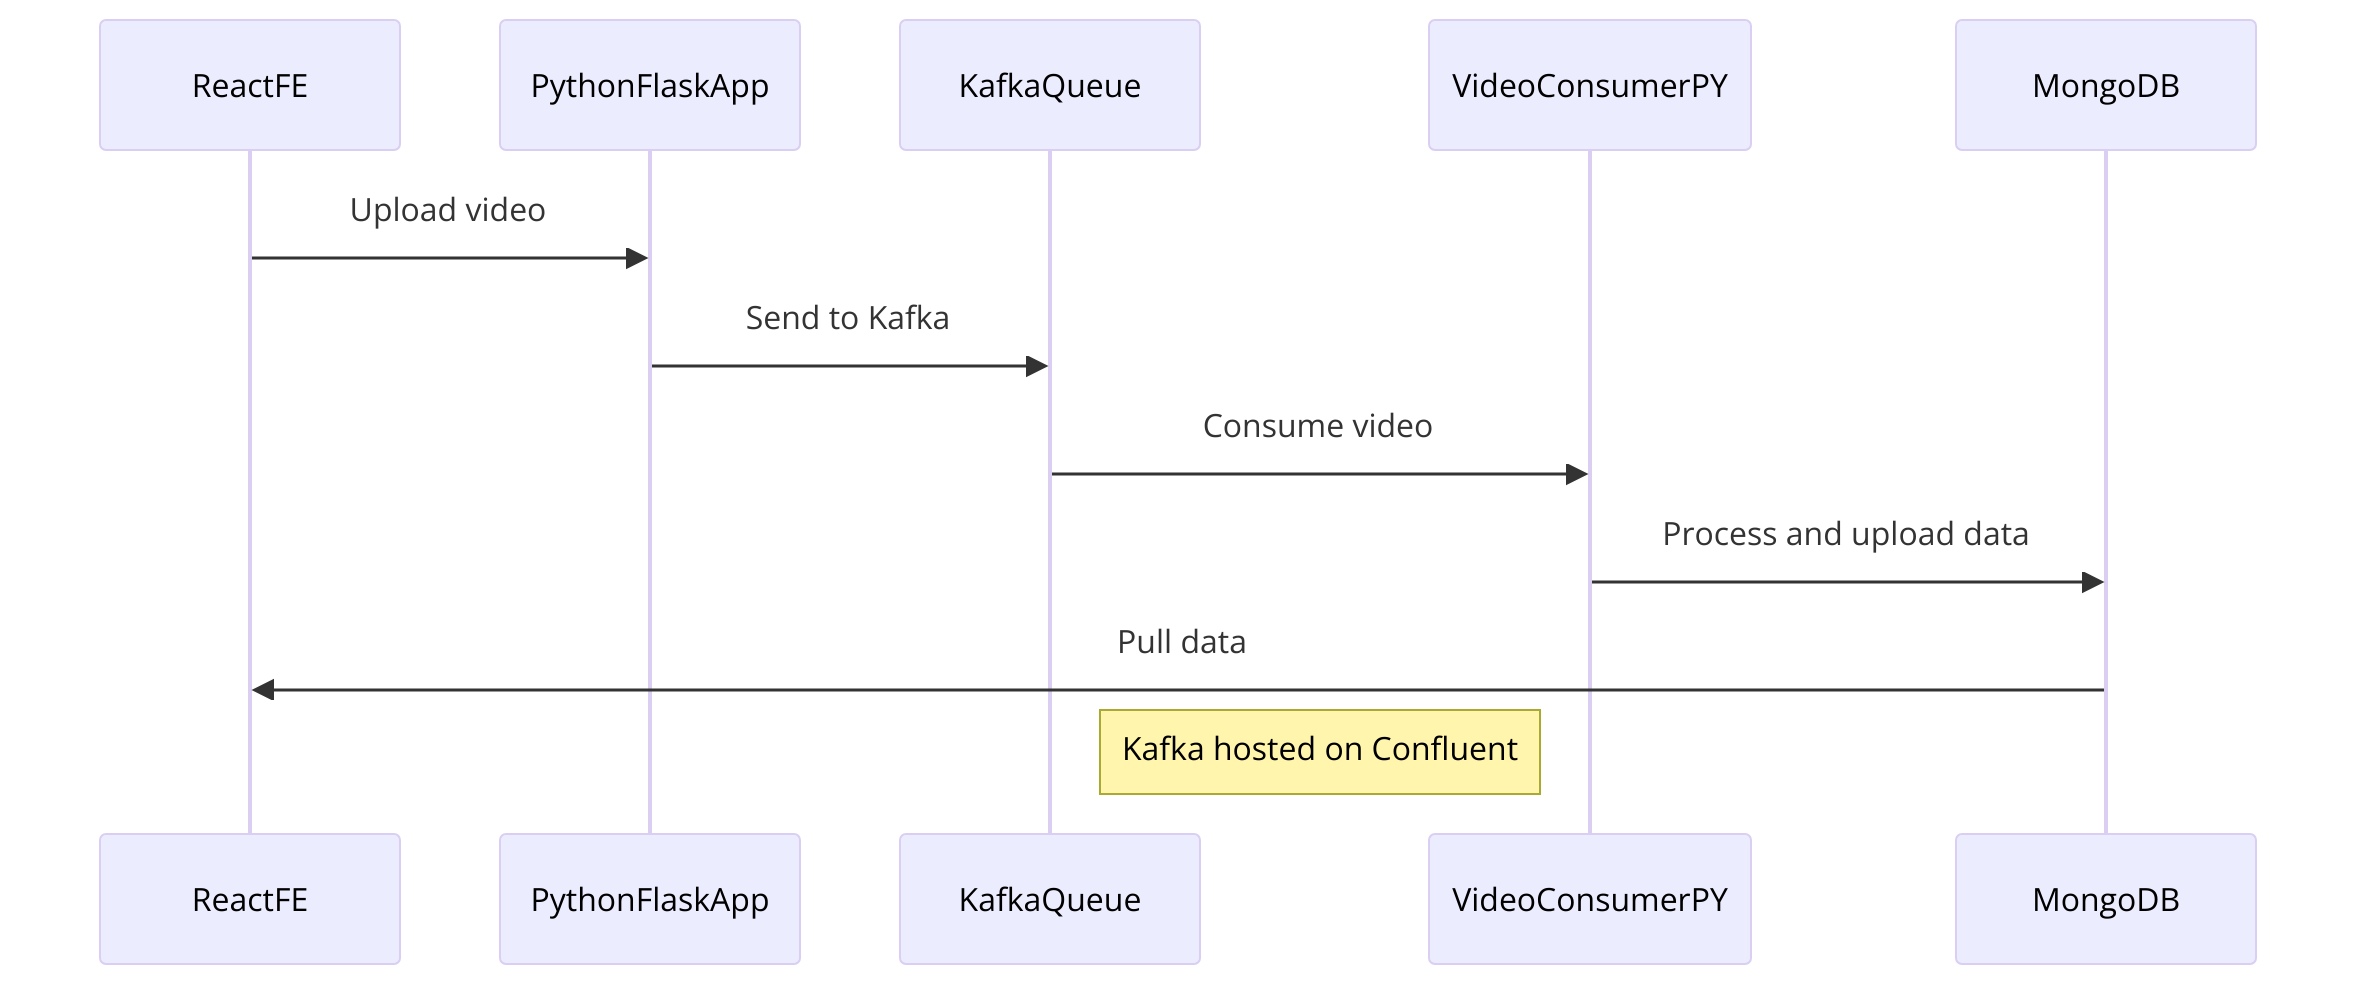
\includegraphics[width=0.9\textwidth]{images/systemFlowChart.png}
    \caption{Flowchart\cite{lucidchartDataFlow} of TrafficVision System Operations.}
    \label{fig:systemFlowChart}
\end{figure}


\section{TrafficVision System Architecture}

\subsection{Frontend Deployment}
The frontend of TrafficVision is constructed using React, a  JavaScript library for building user interfaces. The choice of React is attributed to its component-based architecture, which facilitates the development of interactive UIs.
\begin{itemize}
    \item Users use this frontend to upload traffic videos and additional data into the system, initiating the data processing workflow.
\end{itemize}

\subsection{Serverless Deployment: Processing Server}
Upon user interaction with the frontend, video and data uploads trigger actions within a serverless processing server.
\begin{itemize}
    \item The serverless model, functioning as a function-as-a-service (FaaS), dynamically executes backend code in response to events, in this scenario, video uploads, circumventing the need for a persistent server environment.
    
    \item The processing server operates on a Python runtime, renowned for its extensive libraries that support a multitude of web and data processing functionalities.
    
    \item Within this server, two technologies are utilized:
    \begin{itemize}
        \item \textbf{YOLOv8 (You Only Look Once):} This state-of-the-art deep learning algorithm specializes in object detection within video frames in real-time, identifying vehicles and other objects promptly and accurately.
        
        \item \textbf{Apache Kafka:} A robust distributed event streaming platform that orchestrates real-time data feeds. Kafka manages the flow of data throughout the system components, particularly by queuing video processing tasks efficiently.
    \end{itemize}
\end{itemize}

\subsection{Cloud Database: MongoDB}
Post-processing of video data, MongoDB, a NoSQL cloud database, is employed to manage the data output.
\begin{itemize}
    \item MongoDB is chosen for its adaptable, schema-less data structure and powerful scalability, which is ideal for handling the vast and varied datasets of TrafficVision.
    
    \item The database serves as a repository for processed traffic data, which can be later fetched by the frontend for display and analysis purposes.
\end{itemize}

\subsection{Kafka Deployment on Confluent}
Apache Kafka's deployment within the TrafficVision system is facilitated through Confluent, which is a fully managed Kafka service that simplifies the process of running Kafka.

The following snippet of code simplifies the Kafka configuration for connecting to the Confluent service:

\begin{verbatim}
kafka_config = {
    "bootstrap.servers": os.getenv("KAFKA_BROKER_URL"),
    "security.protocol": "SASL_SSL",
    "sasl.mechanisms": "PLAIN",
    "sasl.username": os.getenv("KAFKA_API_KEY"),
    "sasl.password": os.getenv("KAFKA_API_SECRET"), 
    ...
}
\end{verbatim}

This configuration uses the Producer and Consumer components ensuring they communicate efficiently with the Kafka cluster hosted on Confluent. The TrafficVision system uses Confluent's managed Kafka solution to ensure high-throughput data processing and streamlining the real-time video analytics pipeline.

\subsection{Data Flow}
The operation of TrafficVision encompasses a series of coordinated processes:
\begin{itemize}
    \item \textbf{Video Upload:} Utilizing the frontend application, users upload videos to the processing server, instigating an event that forwards the video and associated data to the server for processing.
    
    \item \textbf{Data Processing:} Leveraging serverless deployment, video data is processed in real-time. Kafka's queuing system allows for scalable and parallel processing of multiple video streams.
    
    \item \textbf{Data Storage:} Upon processing the data is stored in MongoDB, making it accessible for subsequent retrieval.
    
    \item \textbf{Data Retrieval:} The React-based frontend retrieves processed video data from MongoDB, presenting users with comprehensive traffic analysis and insights.
\end{itemize}

\begin{figure}[H]
    \centering
    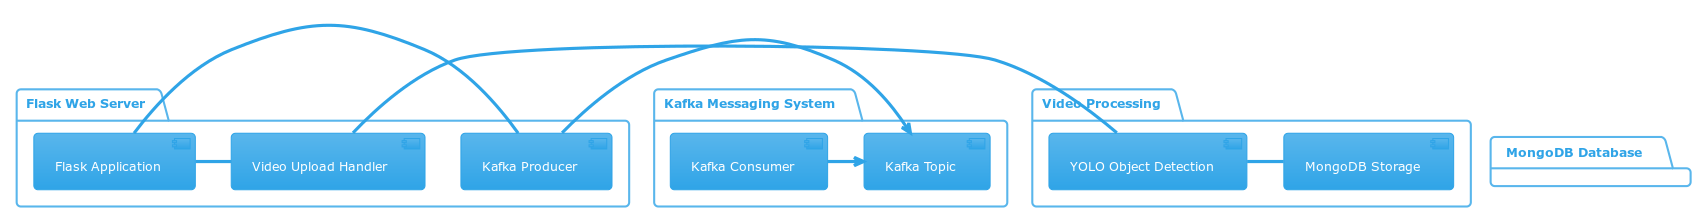
\includegraphics[width=0.9\textwidth]{images/mapDiagram.png}
    \caption{Map Diagram of the TrafficVision Data Flow.}
    \label{fig:mapDiagram}
\end{figure}


\section{Component Interaction and Code Correlation}

The TrafficVision system's UML\cite{umlDiagramMiro} diagram provides a detailed overview of the component interactions within the architecture. The diagram is essential in understanding the system's modularity and connectivity between components.

\subsection{Flask Application}

The \texttt{FlaskApplication} acts as the interface for client interactions. It handles HTTP requests including video uploads and assigns tasks to other components. The following code snippet represents the video upload handling within the Flask application, corresponding to the \texttt{route} method in the UML class:

\begin{verbatim}
@app.route("/upload", methods=["POST"])
def upload_video():
    # [Code to handle video upload]
\end{verbatim}

\subsection{Kafka Producer}

The \texttt{Producer} sends messages to the Kafka cluster. Upon a successful video upload the producer sends a message containing the video ID and metadata, as shown in the code below:

\begin{verbatim}
try:
    producer.produce("incoming-videos", key=str(uuid.uuid4()), value=message)
    producer.flush()
except Exception as e:
    # [Error handling code]
\end{verbatim}

\subsection{YOLO Object Detection}

The \texttt{YOLO} class represents the object detection component using the YOLOv8 algorithm. The code snippet below shows the model loading and video processing, which correlates with the UML diagram:

\begin{verbatim}
model = YOLO("yolov8n.pt")
# [Code to process video and detect objects]
\end{verbatim}

\subsection{MongoDB Storage}

The \texttt{MongoClient} handles data storage in MongoDB. The process of inserting data into the database is represented in the following snippet:

\begin{verbatim}
if info_list:
    collection.insert_many(info_list)
    # [Code to handle database insertion]
\end{verbatim}

\subsection{Integration and Workflow}

Integrating these components allows for a seamless flow from video upload to object detection and data storage. The provided code offers a concrete implementation of the conceptual UML structure.

\begin{figure}[H]
    \centering
    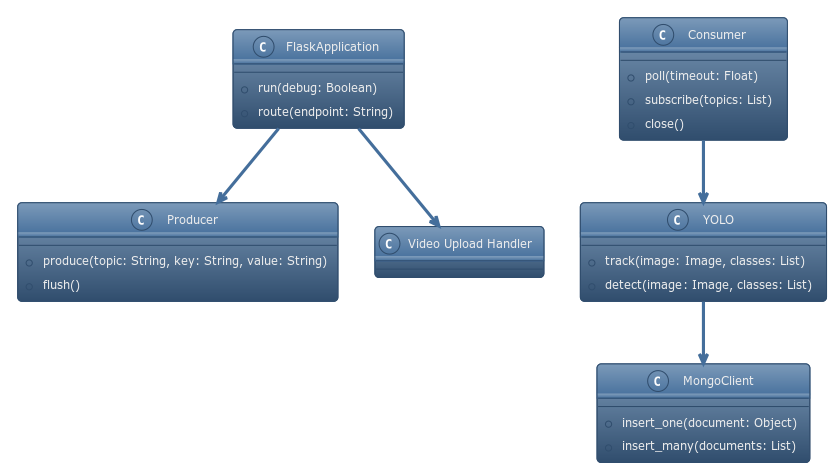
\includegraphics[width=0.9\textwidth]{images/uml.png}
    \caption{UML Diagram of TrafficVision Components.}
    \label{fig:umlDiagram}
\end{figure}

This UML diagram showcases the individual responsibilities of each system component and its modularity within TrafficVision for efficient traffic video processing and analysis.


\section{Environment Configuration with \texttt{.env} Files}

\subsection{Purpose and Benefits}

The TrafficVision system uses \texttt{.env}\cite{gentleIntroductionEnvFiles} files to manage environment variables, which are crucial for defining the runtime environment configuration outside of the codebase. This approach separates configuration from code, which is a principle of a twelve-factor app methodology\cite{twelveFactor} leading to several advantages:

\begin{itemize}
    \item \textbf{Security:} Sensitive information such as API keys and database credentials are kept out of the version control system reducing the risk of security breaches.
    \item \textbf{Portability:} Developers can create multiple \texttt{.env} files for different environments like development, testing and production making it easier to manage and deploy the application across various environments.
    \item \textbf{Customization:} Each instance of the application can be easily customized by changing the environment variables without altering the code.
\end{itemize}

\subsection{Implementation in TrafficVision}

The TrafficVision system utilizes the \texttt{dotenv} library for Python to load the configuration variables from the \texttt{.env} file when the application starts. The following code snippet shows how the environment variables are loaded:

\begin{verbatim}
from dotenv import load_dotenv
DOTENV_PATH = "./.env"
load_dotenv(dotenv_path=DOTENV_PATH)
\end{verbatim}

This simple yet effective setup allows the application to access the environment variables as needed, for instance:

\begin{verbatim}
kafka_config = {
    "bootstrap.servers": os.getenv("KAFKA_BROKER_URL"),
    ...
    "sasl.password": os.getenv("KAFKA_API_SECRET"),
}
\end{verbatim}

In this example the Kafka connection configuration is built using values sourced from the environment which allows for flexibility and security.

\subsection{Implication}
TrafficVision's system design utilizes cutting edge technologies and practices to make a flexible and effective traffic management solution. Front and center of its frontend is React's user friendly user interface, where traffic information can be uploaded. This user interaction launches a backend response in the backend which handles video data uploads dynamically.

YOLOv8's real time object detection and Apache Kafka's information streaming are central to the system processing abilities, all hosted in the scalable Confluent managed services environment. These technologies work together to provide quick and precise processing of traffic videos, queuing activities and smartly managing information flows.

Persistence and results of processed information are handled by MongoDB, a NoSQL cloud database with adaptable data structure and scalability which successfully handles the different produced data sets.

TrafficVision's environment configuration approach based on.env documents highlights the system's operational flexibility and security. By externalizing configuration detail, TrafficVision secures very sensitive information and offers flexibility to adapt to various deployment environments without refactoring the core codebase.

To sum up, TrafficVision's system architecture is a mix of intuitive user interfaces, serverless backend computing, information processing, and configuration management security. This sophisticated integration allows TrafficVision to offer effective traffic analysis.